% --------------------------------------------------------------
% This is all preamble stuff that you don't have to worry about.
% Head down to where it says "Start here"
% --------------------------------------------------------------
 
\documentclass[12pt]{article}
 
\usepackage[margin=1in]{geometry} 
\usepackage{amsmath,amsthm,amssymb}
\usepackage{xcolor}
\usepackage{listings}
\usepackage{graphicx}
\usepackage{hyperref}
\usepackage{listings}
\usepackage{stackengine}
\usepackage{array}
\graphicspath{{/home/arpit/Desktop/iitd/sem_7/COL334/projects/Getting-To-Know-Network-Traffic/img}}

\newcommand{\N}{\mathbb{N}}
\newcommand{\Z}{\mathbb{Z}}
 
\newenvironment{theorem}[2][Theorem]{\begin{trivlist}
\item[\hskip \labelsep {\bfseries #1}\hskip \labelsep {\bfseries #2.}]}{\end{trivlist}}
\newenvironment{lemma}[2][Lemma]{\begin{trivlist}
\item[\hskip \labelsep {\bfseries #1}\hskip \labelsep {\bfseries #2.}]}{\end{trivlist}}
\newenvironment{exercise}[2][Exercise]{\begin{trivlist}
\item[\hskip \labelsep {\bfseries #1}\hskip \labelsep {\bfseries #2.}]}{\end{trivlist}}
\newenvironment{problem}[2][Problem]{\begin{trivlist}
\item[\hskip \labelsep {\bfseries #1}\hskip \labelsep {\bfseries #2.}]}{\end{trivlist}}
\newenvironment{question}[2][Question]{\begin{trivlist}
\item[\hskip \labelsep {\bfseries #1}\hskip \labelsep {\bfseries #2.}]}{\end{trivlist}}
\newenvironment{corollary}[2][Corollary]{\begin{trivlist}
\item[\hskip \labelsep {\bfseries #1}\hskip \labelsep {\bfseries #2.}]}{\end{trivlist}}

\newenvironment{solution}{\begin{proof}[Solution]}{\end{proof}}
\definecolor{codegreen}{rgb}{0,0.6,0}
\definecolor{codegray}{rgb}{0.5,0.5,0.5}
\definecolor{codepurple}{rgb}{0.58,0,0.82}
\definecolor{backcolour}{rgb}{0.95,0.95,0.92}

\lstdefinestyle{mystyle}{
    backgroundcolor=\color{backcolour},   
    commentstyle=\color{codegreen},
    keywordstyle=\color{magenta},
    numberstyle=\tiny\color{codegray},
    stringstyle=\color{codepurple},
    basicstyle=\ttfamily\footnotesize,
    breakatwhitespace=false,         
    breaklines=true,                 
    captionpos=b,                    
    keepspaces=true,                 
    numbers=left,                    
    numbersep=5pt,                  
    showspaces=false,                
    showstringspaces=false,
    showtabs=false,                  
    tabsize=2
}
\lstset{style=mystyle}
\begin{document}
 
% --------------------------------------------------------------
%                         Start here
% --------------------------------------------------------------
 
\title{Assignment 1: Getting to Know Network Traffic}
\author{Arpit Prasad\\ 
COL334: Computer Network}

\maketitle
\section{Measurement Tools}

\subsection{ping}

\begin{figure}[h!]
    \centering
    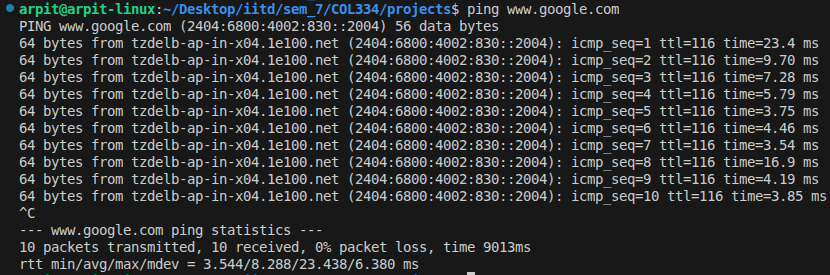
\includegraphics[width=0.8\textwidth]{google_ping.png}
    \caption{Ten Pings to google.com}
\end{figure}

\begin{figure}[h!]
    \centering
    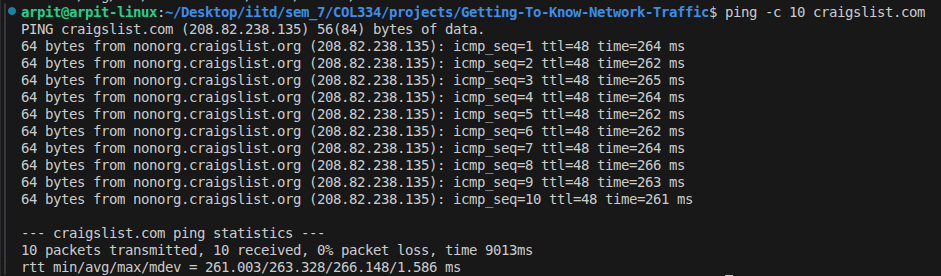
\includegraphics[width=0.8\textwidth]{craigslist_ping.png}
    \caption{Ten Pings to craigslist.com}
\end{figure}

\begin{enumerate}
    \item \textbf{Protocols Used}: Ping uses ICMP protocol. It sends the Echo Request packet to the destination host and recieves Echo Reply packet from the same. It sits on the third layer of the protocol stack, which is the network layer.
    \item \textbf{Latency}:
    \begin{enumerate}
        \item \textbf{Avg Latency of Craigslist}: 263.328 ms
        \item \textbf{Avg Latency of Google}: 30.543 ms
        \item Google's host has \textbf{smaller RTT} than Craigslist
        \item \textbf{Reason for different latencies of websites}:
        \begin{enumerate}
            \item Google has more number of hosts than Craigslist, which splits newtwork traffic
            \item Google's traffic might directly peer with most of the ISPs in the same tier of internet hierarchy (Regional IPSs).
            % \item Physical distance to Google's host is lesser than Craigslist's host, hence reaching the destination host earlier. (Craigslist has a host in San Fransico, whereas, Google's hosts are distributed all across the world, as well as in India, hence smaller RTT)
        \end{enumerate}
        \item \textbf{Reason for differnt latencies across pings for same website}:
        \begin{enumerate}
            \item Length of Queue for service at destination host is not constant in time and varies according to the number of user who requested for service before we place any request (queueing of packets, at the host)
            \item Network congestion is not constant, hence each switch in the network may not have same number of packets it has to route across differnt time
            \item Differnt routes may be taken for different pings leading to different paths and hence latencies
        \end{enumerate}
    \end{enumerate}
    \item \textbf{Using IPv6 for both websites}
    \begin{figure}[h!]
        \centering
        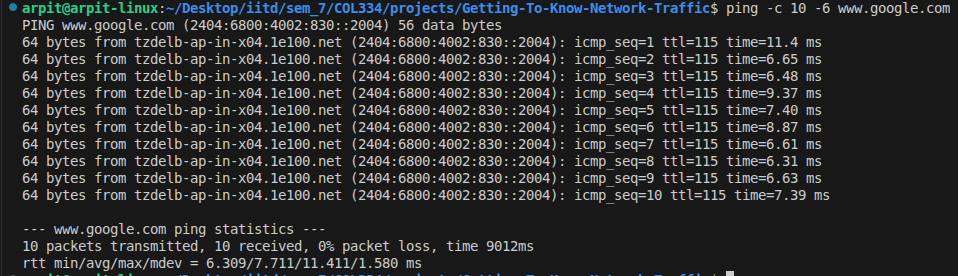
\includegraphics[width=0.8\textwidth]{google_ping_6.png}
        \caption{Ten Pings to www.google.com using IPv6}
    \end{figure}
    \begin{figure}[h!]
        \centering
        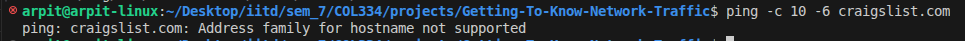
\includegraphics[width=0.8\textwidth]{craigslist_ping_6.png}
        \caption{Error when pinging craigslist.com}
    \end{figure}
    \begin{enumerate}
        \item \textbf{How to force IPv6}: pass a flag -6 to force ping to follow IPv6
        \item \textbf{Result}: IPv6 was supported by Google's host but not by Craigslist's host
        \item \textbf{Why $ping -6$ Failed for Craigslist's host}: 
        \begin{enumerate}
            \item When checking the IPv6 address for craigslist.com using dig AAAA craigslist.com, my computer does not find any IPv6 address as can be seen from Fig. 5, hence does not know which address to resolve to. Therefore, forcing ping to follow IPv6 Addresing cannot be executed.
            \item Also, since IPv6 worked for Google's host, implies that my computer and Google's host both support IPv6. If a failure of Address Family support has occured it must have occured on Craigslist's server. This implies Craigslist's server does not support IPv6 addresses.
        \end{enumerate}
    \end{enumerate}
    \item \textbf{Max size of the packets}
    % \begin{table}[h!]
    %     \centering
    %     \caption{Max Size of Data Transmitted from Ping, practically obtained by experiment}
    %     \begin{tabular}{|c|c|c|c|}
    %         \hline
    %         Host & Max Message Size & ICMP Header Size & Max Total Size \\
    %         \hline
    %         www.google.com & 1462 bytes & 8 bytes & 1470 bytes \\
    %         craigslist.com & 283 bytes & 28 bytes & 311 bytes \\
    %         \hline
    %     \end{tabular}
    % \end{table}
    % \begin{enumerate}
    %     \item Reason of Limit to Size: The network interfaces have a Maximum Transmission Unit for precautions (not to overload a server or a network device, which would disallow the timely servicing of all packets), that limit the packet size. Hence the bottleneck in the path is the device with the smallest Maximum Transmission Unit 
    %     \item The packet size may also be limited by the OS
    %     \item For IPv6 over ethernet networks is limited ideally to 1500 bytes, but Table 1 shows what was practically achieved 
    %     \item The difference between practical and ideal may be caused by a network device through which the packet was routed has smaller Maximum Transmission Unit.
    %     \item To send a larger packet size, the packet must be fragmented
    % \end{enumerate}
    \begin{enumerate}
        \item Max Size = 65535 bits
        \item The length of the field - "total length" in the packet structure - which indicates the size of the payeload, 16 for both IPv4 and IPv6 Addressing in ping packets. Hence, the total payload size = $2^{16} - 1$ (the 1 excludes all bits zero) = 65535 bits. Theoretically, the protocol allows these many number of bits to be sent as data in the payload.
    \end{enumerate}
\end{enumerate}

\subsection{traceroute}
\begin{enumerate}
    \item IPv4 Address for www.google.com : 172.217.26.110
    \item IPv4 Address for craigslist.com : 208.82.238.135
\end{enumerate}

\begin{figure}[h!]
    \centering
    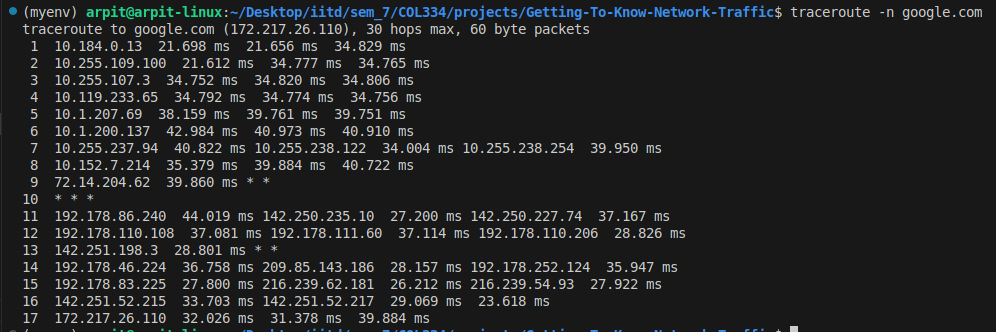
\includegraphics[width=0.8\textwidth]{google_tr.png}
    \caption{Trace Route of sending packet to www.google.com}
\end{figure}

\begin{figure}[h!]
    \centering
    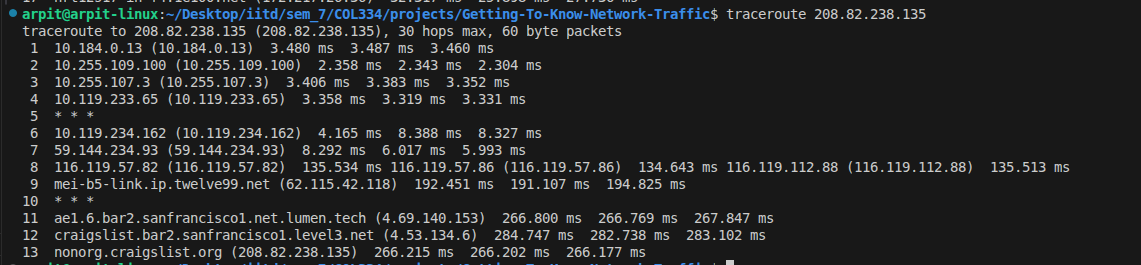
\includegraphics[width=0.8\textwidth]{craigslist_tr.png}
    \caption{Trace Route of sending packet to craigslist.com}
\end{figure}
\renewcommand{\labelenumi}{\Alph{enumi}}
\begin{enumerate}
    \item \textbf{Number of Hops}:
    \begin{table}[h!]
        \centering
        \caption{Number of Hops for Websites}
        \begin{tabular}{|c|c|}
            \hline
            Host & Number of Hops \\
            \hline
            www.google.com & 17 \\
            craigslist.com & 13 \\
            \hline
        \end{tabular}
    \end{table}
    \begin{figure}[h!]
        \centering
        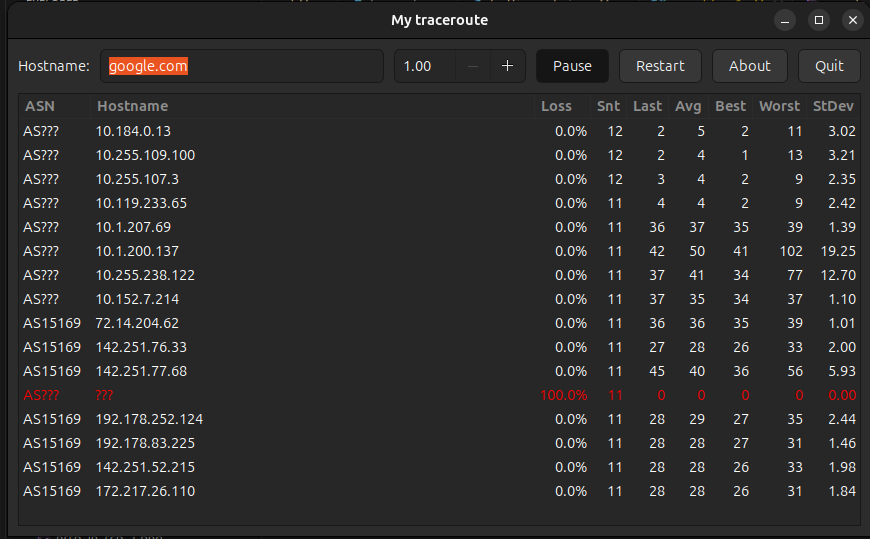
\includegraphics[width=0.8\textwidth]{google_asn.png}
        \caption{Autonomous System Number (denoted as ASN here) for each IP Address in the trace route of www.google.com (produces using the tool: mtr)}
    \end{figure}
    \begin{figure}[h!]
        \centering
        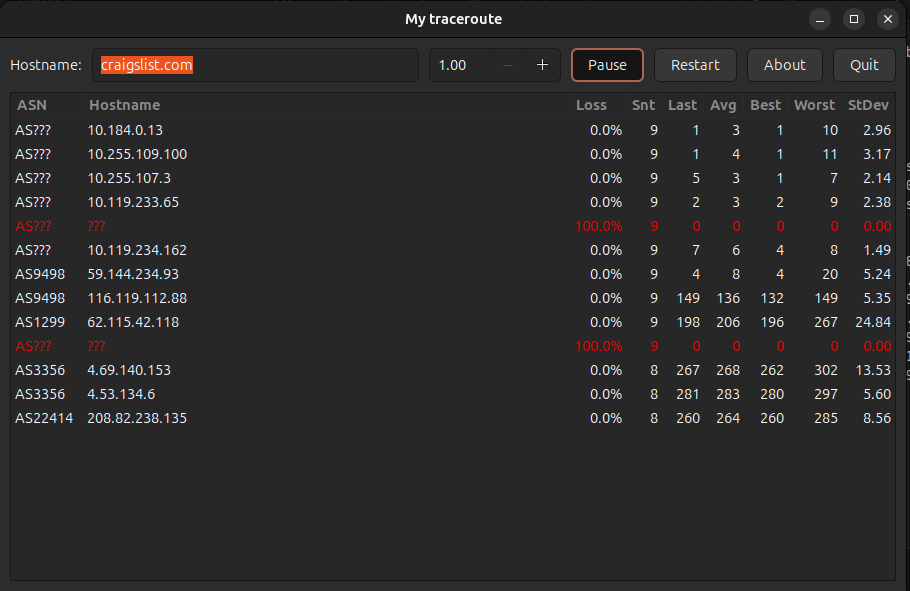
\includegraphics[width=0.8\textwidth]{craigslist_asn.png}
        \caption{Autonomous System Number (denoted as ASN here) for each IP Address in the trace route of craigslist.com (produces using the tool: mtr)}
    \end{figure}
    \item \textbf{Explanation for "*"}: Some servers do not cater to traceroute packets, for security reasons and traffic control, hence do not send the Time Exceeded packet back to the source and hence, we do not have information about this node. This is represented in the traceroute by "*"
    \item \textbf{Multiple IP Addresses for the same Hop Count}: $traceroute$ sends three packets for each hop. The three packets may opt for independent routes, depending on the congestion of the network. traceroute lists all the unique ip addresses of the nodes encountered by the three packets
    \item The following tables (Table 2 for google.com and Table 3 for craigslist.com) \textbf{lists the IP Addresses and their correspoding RTTs and Geolocations}
    \begin{table}[h!]
        \centering
        \caption{IP Addresses and their GeoLocations for google.com. Note: NA means Not Available from the respective method listed in the column}
        \resizebox{\linewidth}{!}{
        \begin{tabular}{|c|c|>{\centering\arraybackslash}m{0.5\textwidth}|>{\centering\arraybackslash}m{0.5\textwidth}|>{\centering\arraybackslash}m{0.5\textwidth}|c|}
            \hline
            \textbf{Sl No} & \textbf{IP Address} & \textbf{DNS} & \textbf{DNS Geolocation} & \textbf{Maxmind Geolocation} & \textbf{RTT} (ms) \\
            \hline
            % 1 & 10.194.0.1 & NA & NA & NA 6.100 \\
            % 2 & 10.254.238.1 & NA & NA & NA & 6.087 \\
            % 3 & 10.255.107.3 & NA & NA & NA & 21.154 \\
            % 4 & 10.119.233.65 & NA & NA & NA & 21.147 \\
            % 5 & 10.1.207.69 & NA & NA & NA & 37.188 \\
            % 6 & 10.1.200.137 & NA & NA & NA & 50.264 \\
            % 7 & 10.255.237.94 & NA & NA & NA & 115.352 \\
            % 8 & 10.152.7.214 & NA & NA & NA & 215.550 \\
            % 9 & 72.14.204.62 & NA & NA & United States (US), North America & 215.512 \\
            % 10 & NA & NA & NA & NA \\
            % 11 & 142.250.214.102 & NA & NA & United States (US), North America & 186.456 \\
            % 12 & 142.251.77.68 & NA & NA & United States (US), North America & 151.676 \\
            % 13 & 142.251.197.253 & NA & NA & United States (US), North America & 33.512 \\
            % 14 & 142.251.247.50 & NA & NA & United States (US), North America & 36.570 \\
            % 15 & 192.178.83.215 & NA & NA & United States (US), North America & 59.573 \\
            % 16 & 142.251.49.115 & NA & NA & United States (US), North America & 45.122 \\
            % 17 & 172.217.26.36 & nrt12s17-in-f4.1e100.net or nrt12s17-in-f36.1e100.net or tzdelb-ap-in-f4.1e100.net & Narita, Japan, Tanzania & United States (US), North America & 48.186 \\

            1 & 10.184.0.13 & NA & NA & NA & 8.457 \\
            2 & 10.255.109.100 & NA & NA & NA & 9.288 \\
            3 & 10.255.107.3 & NA & NA & NA & 9.235 \\
            4 & 10.119.233.65 & NA & NA & NA & 9.184 \\
            5 & 10.1.207.69 & NA & NA & NA & 37.041 \\
            6 & 10.1.200.137 & NA & NA & NA & 42.454 \\
            7 & 10.255.238.122 & NA & NA & NA & 34.988 \\
            8 & 10.152.7.214 & NA & NA & NA & 37.466 \\
            9 & * & NA & NA & NA & * \\
            10 & * & NA & NA & NA & * \\
            11 & 72.14.233.58 & NA & NA & United States (US), North America & 39.810 \\
            12 & 192.178.110.204 & NA & NA & United States (US), North America & 27.622 \\
            13 & * & NA & NA & NA & 142.251.198.3 \\
            14 & 192.178.252.110 & NA & NA & United States (US), North America & 31.866 \\
            15 & 216.239.54.93 & NA & NA & United States (US), North America & 34.751 \\
            16 & 142.251.52.215 & NA & NA & United States (US), North America & 26.822 \\
            17 & 172.217.26.110 & kix05s01-in-f14.1e100.net or kix05s01-in-f110.1e100.net or tzdelb-bj-in-f14.1e100.net & Osaka Japan or Tanzania & United States (US), North America & 27.744 \\
            \hline
        \end{tabular} }
    \end{table}
    \begin{table}[h!]
        \centering
        \caption{IP Addresses and their GeoLocations for craigslist.com. Note: NA means Not Available from the respective method listed in the column}
        \resizebox{\linewidth}{!}{
        \begin{tabular}{|c|c|c| >{\centering\arraybackslash}m{0.5\textwidth} | >{\centering\arraybackslash}m{0.5\textwidth} |c|c|}
            \hline
            \textbf{Sl No} & \textbf{IP Address} & \textbf{DNS} & \textbf{DNS Geolocation} & \textbf{Maxmind Geolocation} & \textbf{RTT} (ms) \\
            \hline
            1 & 10.184.0.13 & NA & NA & NA & 685.733 \\
            2 & 10.255.109.100 & NA & NA & NA & 685.597 \\
            3 & 10.255.107.3 & NA & NA & NA & 685.551 \\
            4 & 10.119.233.65 & NA & NA & NA & 685.507 \\
            5 & * & NA & NA & NA & * \\
            6 & 10.119.234.162 & NA & NA & NA & 685.376 \\
            7 & 59.144.234.93 & NA & NA & Bengaluru, Karnataka, India & 5.715 \\
            8 & 116.119.112.88 & NA & NA & India & 138.551 \\
            9 & 62.115.42.118 & mei-b5-link.ip.twelve99.net & Meridian, Mississippi, USA & France & 197.050 \\
            10 & * & NA & NA & NA & * \\
            11 & 4.69.140.153 & ae1.6.bar2.SanFrancisco1.net.lumen.tech & San Francisco, California, United States (US), North America & United States, North America & 268.401 \\
            12 & 4.53.134.6 & CRAIGSLIST.bar2.SanFrancisco1.Level3.net & San Francisco, California, United States (US), North America & San Francisco, California, United States (US), North America & 270.387 \\
            13 & 208.82.238.135 & nonorg.craigslist.org & San Francisco, California, United States (US), North America & San Francisco, California, United States (US), North America & 259.620 \\
            \hline
        \end{tabular}}
    \end{table}

    \begin{enumerate}
        \item \textbf{For google.com} : most of the network devices that relay the packet are private and hence no information is obtained about them. However we observe a delta in 9th hop, therefore we can assume that the packet has crossed the country.
        \item \textbf{For craigslist.com} : The bigger deltas are observed when there is a change in country. For eg., from Table 4, we observe that upto Bangalore the RTT was 5.77 ms but as the relay proceeded to the US, the RTT becomes signficanly higher, 197.05 ms. 
    \end{enumerate}

    Hence, from the above explanation, the data intuitively makes sense.
    
    \item \textbf{Three Tier Architecture}:
    \begin{enumerate}
        \item \textbf{craigslist.com} : Here we observe the three tier architecture clearly. Since first the packet travels from Delhi to Bangalore (which is a 2nd tier ISP transfer), then the exchange is observed from Bangalore to France and France to San Fransico which are a 1st Tier ISP Transfer. Finally 2nd and 3rd tier transfers occur for the packet to reach craigslist.com server
        \item \textbf{google.com} : Here, we do not observe the three tier architecture clearly. Most of the transfers are through private ip addresses. Google peers its packets in the same level of hierarchy (the Regional ISPs). This is the reason why we observe so many regional ISPs (Unites States (US), North America).
    \end{enumerate}
\end{enumerate}

\section{Network Traffic Collection and Analysis}

\subsection{Traffic Capture}
\renewcommand{\labelenumi}{\Alph{enumi}}
\begin{enumerate}
    \item \textbf{Median Time taken} for the DNS request-response to comlete: \textbf{42.438s}. Note Median was taken on query response times observed in the pcap file when applied with the filter of DNS. (This was done using python script, code present in traffic\_analysis.py)
    \item \textbf{HTTP}
    \begin{enumerate}
        \item \textbf{Number of HTTP Requests} = 363 (fitler used: $http.request$)
        \item \textbf{How webpages are structured}: The webpage is structured like a tree. The root of the tree is the webpage itself. Root's children are the first level abstraction in the webpage, such as the title, the box that contains green ticks (as present in the website httpvshttps.com) etc.. The next level with each abstraction, contains the green ticks itself, in the case of the abstraction mentioned previously. 
        \item \textbf{How browsers render complex pages with multiple images and files}: The browser recursively calls on the nodes of the tree (mentioned above) and fetches the required informaiton, and displays them according to their HTML Code. This way it is able to render complex images and texts. 
    \end{enumerate}
    \item \textbf{TCP Connection}
    \begin{enumerate}
        \item \textbf{Number of TCP Connections} = 31 (filter used: $tcp.flags.syn == 1 and tcp.flags.ack == 0$)
        \item \textbf{Are Number of HTTP Conbnections==Number of TCP Connections}: No, they are generally not equal, however they are related. In one TCP Connection multiple HTTP requests can be made.
        \item \textbf{Content Object Fetch over same TCP Connection}: Yes, some contents gets fetched over the same TCP Connection. This can be supported from the fact that HTTP transfer are made with HTTP/1.1, which implies sustained TCP Connection for multiple HTTP transfers. This was verified using the filter $tcp.stream == 0$ where we checked the upstream flow. This showed multiple to and fro packet flows.
        \begin{figure}[h!]
            \centering
            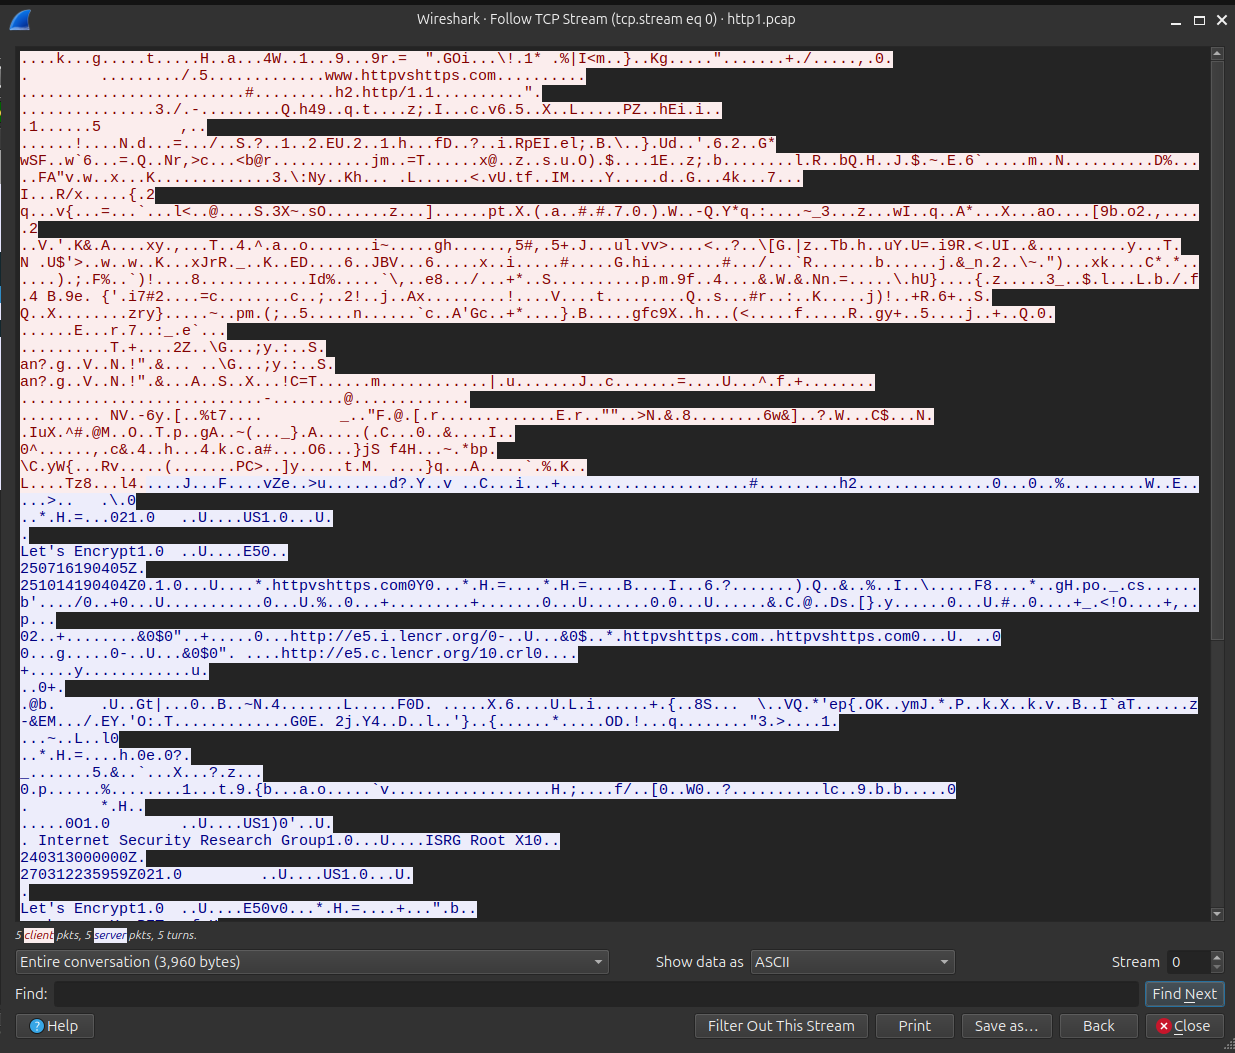
\includegraphics[width=0.8\textwidth]{http_in_tcp_1.png}
        \end{figure}
    \end{enumerate}
    \item \textbf{HTTPs packet trace}
    \begin{enumerate}
        \item \textbf{Is HTTP traffic there?} No, there is no HTTP Traffic (filter used: $http$)
        \item \textbf{Content transfer of HTTP and JavaScript files? and why?}: There is no content tranfer of HTTP and JavaScript. HTTPs is secured data transfer, therefor the file content is encrypted and hence not visible without the key to the file. This is the reason why wireshark does not show this content.
        \item \textbf{dns traffic}: Yes, DNS Traffic is present. DNS is required for look ups to convert web addresses to their correspoding IP Addresses. Once the ip addresses for the websites are resolved no more DNS Traffic is present for that particular domain name. Note: I was able to see DNS traffic because DoH, i.e., DNS over HTTPs is not enabled on my browser. Hence, DNS Traffic could not tunnel through HTTPs. (filter used: $dns$)
        \item \textbf{Number of tcp connections logged} = 7
        \item \textbf{Is Number of TCP Conbnections in HTTPS case == Number of TCP Connections in HTTP case?}: They are not equal. However the HTTPS case has smaller number of TCP Connections. A potential reason is multiplexing, allowing many HTTPS request to be sent simultaneously. Also, apart from TCP Handshake, https use TLS Handshake, which is expensive and hence tend to perform this Handshake lesser number of times. Due to this lesser number of TCP Connections are established.
    \end{enumerate}
\end{enumerate}

\subsection{Performance Analysis}
\begin{enumerate}
    \item[E] \textbf{HTTP vs HTTPs}
    \begin{enumerate}
        \item \textbf{Comparision of time taken for downloads}: HTPP::17.132s and HTTPs::1.614 (93\% faster than HTTP)
        \item \textbf{Observation from the plots}: 
        \begin{enumerate}
            \item The download plot for https.pcap has significant throughput for download in comparision to that for http.pcap. Since the amount of data downloaded is the same, hence if the time of download reduces (as inferred from the time on the website and also the x axis of the plots), this implies throughput increases. The download throughput are upto 100 times more in https than http
            \item Time of downloads can also be justified from the RTT plot. RTT is much smaller in https.pcap case than in comparision to http.pcap. This implies smaller time for data transfers from https.pcap than http.pcap
        \end{enumerate}
         \item \textbf{Assumption for RTT Plots}: We assume no retransmission of signal. Hence, we confirm ACK from the receiver by matching it to the estimated Acknowledgment Number, that is, we find if A == S + L. Here A is the Acknowledgment number received from the receiver, S is the sequence number when the message in consideration was sent to the receiver from the sender and L is the number of bytes of the data.
         \item \textbf{Note}: RTT values are recorded at the time of ACK of the sent message
         \item \textbf{Note}: The images for throughputs have been found for each second {1, 2, 3, ...} on the wall clock
        \begin{figure}[h!]
            \centering
            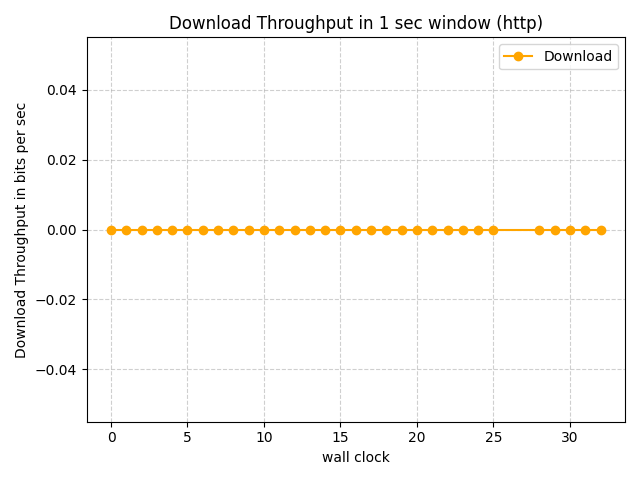
\includegraphics[width=0.8\textwidth]{throughput/to_use/down_throughput.png}
            \caption{Download Throughput using http.pcap}
        \end{figure}
        \begin{figure}[h!]
            \centering
            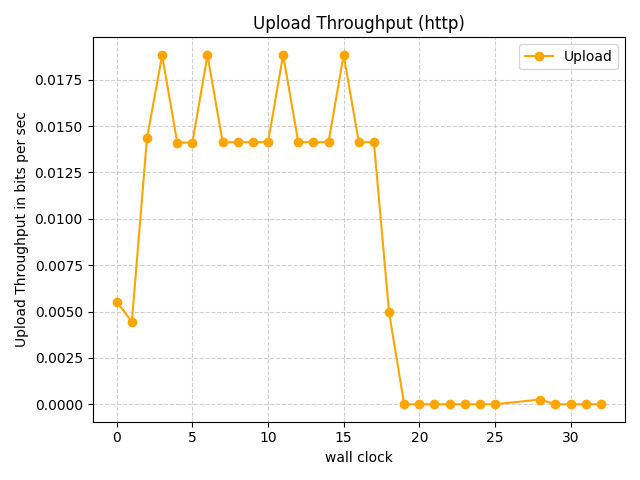
\includegraphics[width=0.8\textwidth]{throughput/to_use/up_throughput.png}
            \caption{Upload Throughput using http.pcap}
        \end{figure}
        \begin{figure}[h!]
            \centering
            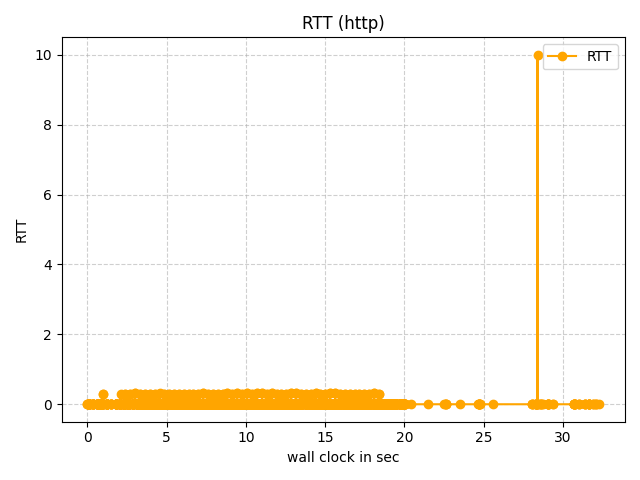
\includegraphics[width=0.8\textwidth]{rtt/to_use/rtt.png}
            \caption{RTT using http.pcap}
        \end{figure}
        \begin{figure}[h!]
            \centering
            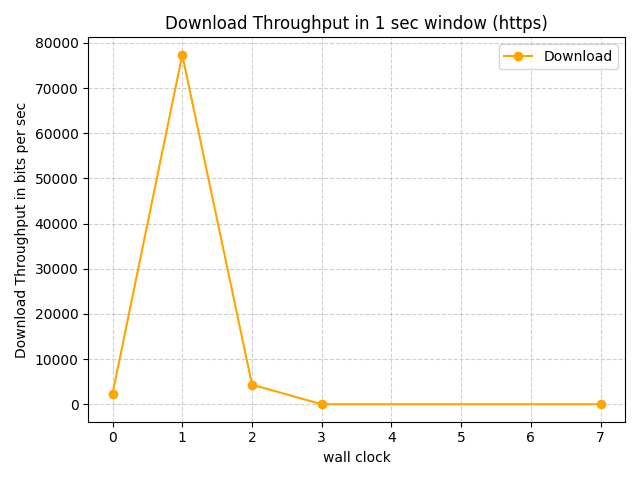
\includegraphics[width=0.8\textwidth]{throughput/to_use/down_throughput_s.png}
            \caption{Download Throughput using https.pcap}
        \end{figure}
        \begin{figure}[h!]
            \centering
            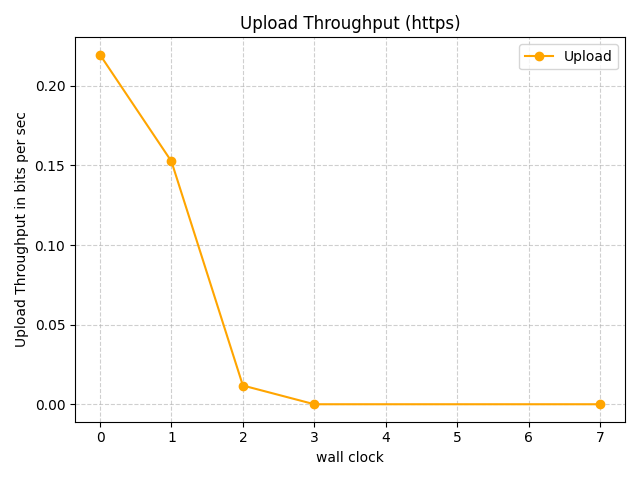
\includegraphics[width=0.8\textwidth]{throughput/to_use/up_throughput_s.png}
            \caption{Upload Throughput using https.pcap}
        \end{figure}
        \begin{figure}[h!]
            \centering
            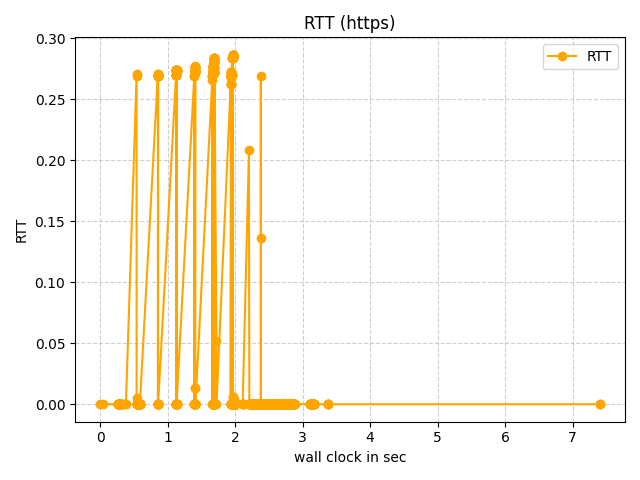
\includegraphics[width=0.8\textwidth]{rtt/to_use/rtt_s.png}
            \caption{RTT using https.pcap}
        \end{figure}
    \end{enumerate}
    
\end{enumerate}
% --------------------------------------------------------------
%     You don't have to mess with anything below this line.
% --------------------------------------------------------------

\end{document}
